\documentclass[8pt]{beamer}
\usefonttheme[onlymath]{serif}


\setbeamertemplate{frametitle}{%
  \vskip1ex
  \usebeamerfont{frametitle}%
  \insertsubsectionhead\par        %  ← 원하는 대로 변경 가능
  \vskip1ex
  \hrule                             % 밑줄(선택)
}

% 테마 선택 (선택 사항)
% \usetheme{Madrid} % 기본 테마, 다른 테마 사용 가능
% \font{serif}
\usepackage{amsfonts}
\usepackage{amssymb}
\usepackage[T1]{fontenc} % To use combination of textbf, textit
\usepackage[dvipsnames]{xcolor}   % can use more variant colors

\usepackage[
  backend=biber,
  style=authoryear,   % or numeric
  citestyle=authoryear
]{biblatex}
\addbibresource{../../references.bib}

\usepackage{subfigure}
\usepackage{subcaption}

% \setcounter{MaxMatrixCols}{20}

% (필요한 패키지들)
% \usepackage{amsthm}
\setbeamertemplate{theorems}[numbered]  % 정리, 정의 등에 번호를 달아줌

% \theoremstyle{plain} % insert bellow all blocks you want in italic
% \newtheorem{theorem}{Theorem}[section] % to number according to section
% 
% \theoremstyle{definition} % insert bellow all blocks you want in normal text
% \newtheorem{definition}{Definition}[section] % to number according to section
% \newtheorem*{idea}{Proof idea} % no numbered block

\newtheorem{proposition}[theorem]{Proposition}

\usepackage{tcolorbox}

% 필요할 경우 패키지 추가
\usepackage{graphicx} % 이미지 삽입을 위한 패키지
\usepackage{amsmath}   % 수식 사용
\usepackage{hyperref}  % 하이퍼링크 추가
\usepackage{cleveref}
\usepackage{multicol}  % 여러 열 나누기
\usepackage{ulem} % 취소선 및줄 나누기



\newcommand{\mrm}[1]{\mathrm{#1}}
\newcommand{\mbb}[1]{\mathbb{#1}}
\newcommand{\mb}[1]{\mathbf{#1}}
\newcommand{\mc}[1]{\mathcal{#1}}
\newcommand{\tb}[1]{\textbf{#1}}
\newcommand{\ti}[1]{\textit{#1}}
\newcommand{\mypois}[1]{\operatorname{Pois}(#1)}

\newcommand{\myber}[1]{\operatorname{Bern}\!\left(#1\right)}
\newcommand{\mybin}[2]{\operatorname{Bin}\!\left(#1,#2\right)}
\newcommand{\mytoinf}[1]{#1 \rightarrow \infty}
\newcommand{\myexp}[1]{\exp{\left(#1\right)}}
\newcommand{\myunif}[2]{\operatorname{Unif}\!\left(#1, #2\right)}
\newcommand{\mygeom}[1]{\operatorname{Geom}\!\left(#1\right)}
\newcommand{\myexpo}[1]{\operatorname{Expo}\!\left(#1\right)}
\newcommand{\abs}[1]{\left\lvert #1 \right\rvert}
\newcommand{\expec}[1]{\operatorname{E}\left[ #1 \right]}
\newcommand{\myvar}[1]{\operatorname{Var}\left[#1\right]}
\newcommand{\myskew}[1]{\operatorname{Skew}\!\left[#1\right]}
\newcommand{\mykurt}[1]{\operatorname{Kurt}\!\left[#1\right]}
\newcommand{\mywei}[2]{\operatorname{Wei}\!\left(#1, #2\right)}
\newcommand{\Span}[1]{\operatorname{Span}\!\left(#1\right)}
\newcommand{\softmax}[2]{\operatorname{softmax}_{#1}\!\left(#2\right)}

% 발표 제목, 저자, 날짜 설정
\title{Dueling DQN}
\author{Gwanwoo Choi}
% \date{}

\begin{document}
% 표지 슬라이드
\begin{frame}
    \titlepage
\end{frame}

% \begin{frame}
%     \frametitle{Table of Contents}
%     \tableofcontents[currentsubsection]
% \end{frame}

\subsection{Double DQN}

\begin{frame}{.}
    Double DQN algorithm is complemented version of previous DQN (\cite{mnih2015human}) and adapts the idea of Double Q-Learning.

    \begin{itemize}
        \item Q-Learning uses Q target $Y^{Q}_t = R_{t+1} + \gamma \max_{a} Q(S_{t+1},a ;\theta)$
        \item Double Q-Learning uses Q target $Y^{\text{Double}Q}_t = R_{t+1} + \gamma Q(S_{t+1}, \max_{a} Q(S_{t+1}, a; \theta_t); \theta_t^\prime)$
    \end{itemize}
\end{frame}

\begin{frame}{.}
    In \cite{van2016deep}, they derived the lower bound of overestimation error.

    \begin{theorem}
        Consider a state $s$ in which all the true optimal action values are equal at $Q^\ast (s,a) = V^\ast (s)$ for some $V^\ast(s)$.
        Let $Q_t$ be arbitrary value estimates that are on the whole unbiased in the sense that $\sum_a (Q_t(s,a) - V^\ast(s)) = 0$, but that are not all correct, such that $\frac{1}{m} \sum_a (Q_t(s,a) - V^\ast(s))^2 = C$ for some $C>0$, where $m  \geq 2$ is the number of actions in $s$.
        Under these conditions, $\max_{a} Q_t(s,a) \geq V^\ast(s) + \sqrt{\frac{C}{m-1}}$
    \end{theorem}

    \bigskip
    \underline{Note that experimentally, the error rather increases.}

    \begin{columns}
        \begin{column}{0.6\textwidth}
            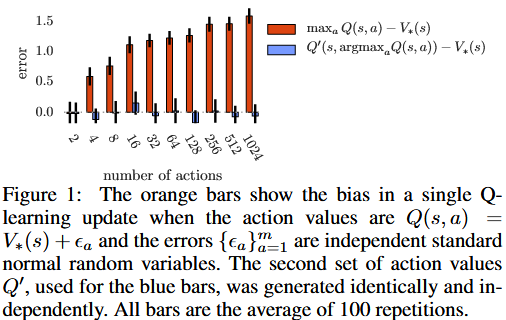
\includegraphics[width=1.0\textwidth]{IncreasingErrorwithNumActions.png}
        \end{column}
        \begin{column}{0.4\textwidth}
            Red bar represents the error of Q-Learning, which shows error increases with the number of actions. Whereas, blue bar represents the error of Double Q-Learning, which implies Double Q-Learning is unbiased.
        \end{column}
    \end{columns}
\end{frame}

\begin{frame}{.}
    In \cite{van2016deep}, there exists another simple toy experiment that reveals overestimation.

    \begin{figure}
        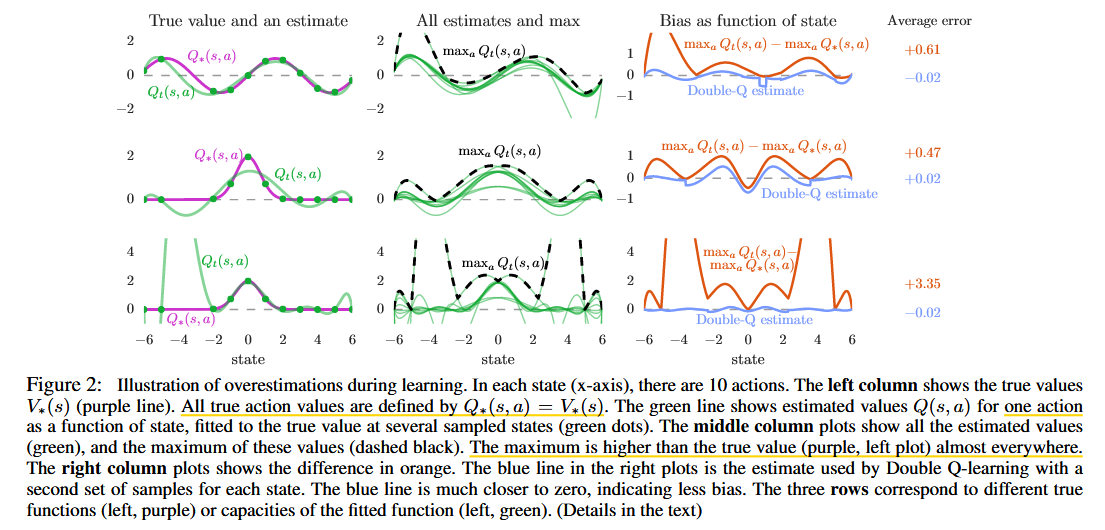
\includegraphics[width=0.8\textwidth]{Figure2.png}
    \end{figure}

    \begin{itemize}
        \item In left column, the purple lines show the true action values.
        \item In middle column, the green lines in each figure shows all action value estimates (there exists 10 actions).
        Black-dotted line shows the maximum action value estimate.
        Green lines in left column show one of the action value estimates of middle column.
        \item In right column, orange line shows difference between purple line and black-dotted line.
        Blue lines, in my guess, show the difference between purple line and estimations of double q-learning.
        \item More details are written in \cite{van2016deep}.
    \end{itemize}
\end{frame}

\begin{frame}{.}
    Above figure shows that overestimations occurs in Q-Learning.
    This overestimations occurs identically in DQN and have negative effects.
    \begin{itemize}
        \item On update, already overoptimistic action values are bootstrapped, leading to even more overoptimistic action values.
        \item Ununiformly overestimated action values between actions leads to pool policy
    \end{itemize}

    \bigskip
    Authors argue combining the idea of Double Q-Learning with DQN can reduce overestimation error.
    \begin{itemize}
        \item The idea of Double Q-Learning is to reduce overestimations by decomposing the max operation in the target into action selection and action evaluation.
    \end{itemize}

    The updtae of Double DQN is the same as for DQN, but replacing the target
    \[
        \begin{gathered}
            Y^{\text{DQN}}_t = R_{t+1} + \gamma \max_{a} Q(S_{t+1}, a; \theta_t^-) \\
            Y^{\text{DoubleDQN}}_t = R_{t+1} + \gamma Q(S_{t+1}, \max_{a}Q(S_{t+1}, a; \theta_t), \theta_t^{-})
        \end{gathered}
    \]
\end{frame}

\begin{frame}{.}
    To show this idea works, authors conducted same experiments as in \cite{mnih2015human}.

    \begin{figure}
        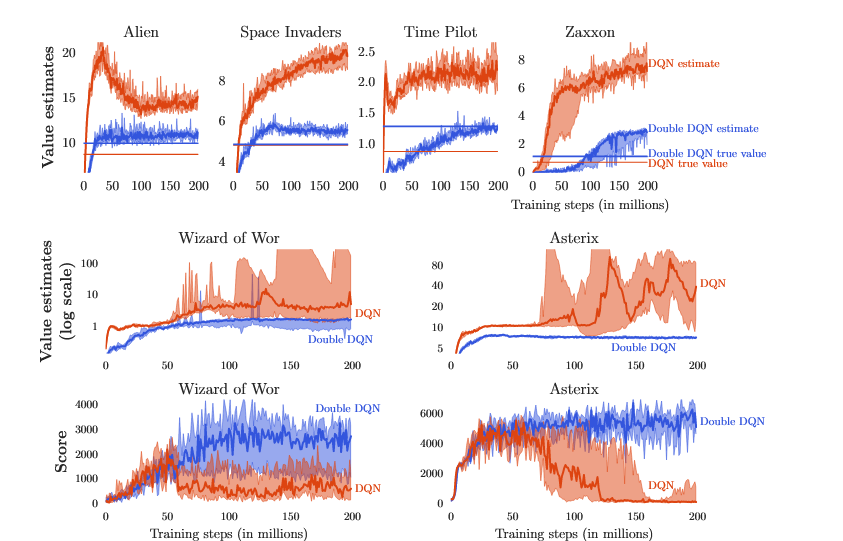
\includegraphics[width=0.75\textwidth]{Figure3.png}
        \caption{Performance of Double DQN on Atari games (Red - DQN, Blue - Double DQN)}
    \end{figure}

    \begin{itemize}
        \item First row shows estimated action values of DQN and Double DQN
        \item Second row shows estimated aciton values \ti{in Log scale}
        \item Last row shows achieved scores of DQN
    \end{itemize}
\end{frame}

\begin{frame}{.}
    \begin{figure}
        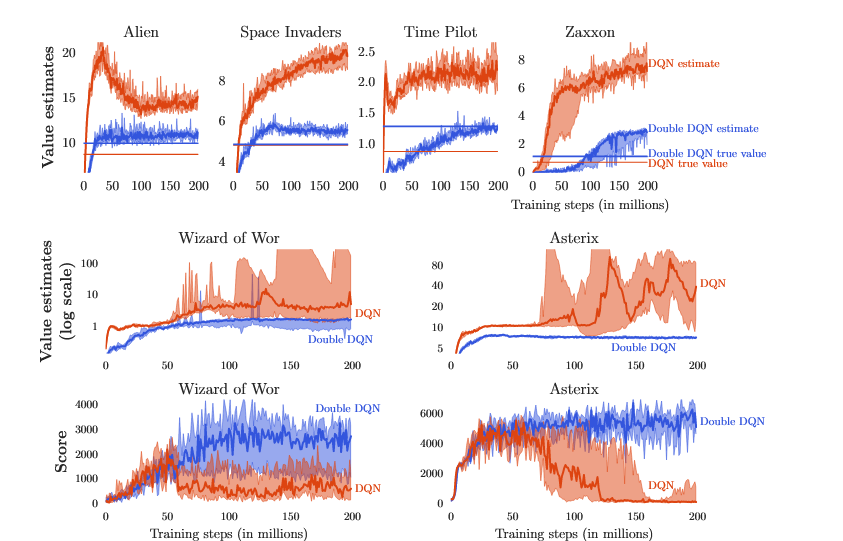
\includegraphics[width=0.75\textwidth]{Figure3.png}
        \caption{Performance of Double DQN on Atari games (Red - DQN, Blue - Double DQN)}
    \end{figure}

    The straight line (ground truth value) is obtained by running the best learned policiesfor several episodes and computing the actual cumulative rewards.

    Note that second and third row are obtained from same games.
    This implies that the overestimations are harming the quality of the resulting policies.
\end{frame}

\begin{frame}{.}
    \begin{figure}
        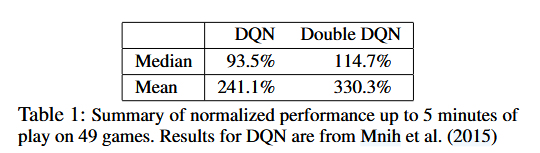
\includegraphics[width=0.65\textwidth]{Table1.png}
    \end{figure}
    \begin{figure}
        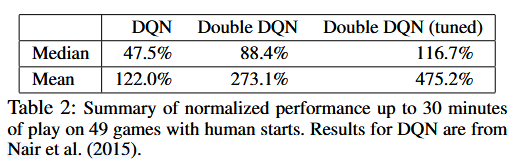
\includegraphics[width=0.65\textwidth]{Table2.png}
    \end{figure}
    Not only Double DQN reduces overestimations, but also it helps generalizing.
    These tables implies that the more takes time to play, the more performance gain is achieved.
    Since as the time goes the environment is vary from starting point, more performance increase in table 2 implies that Double DQN is more robust to the environment change.
\end{frame}

\subsection{References}
\begin{frame}[allowframebreaks]{References}
  \printbibliography
\end{frame}

\end{document}